\documentclass[ST]{subfiles}

\begin{document}
\begin{figure}[h]
\centering
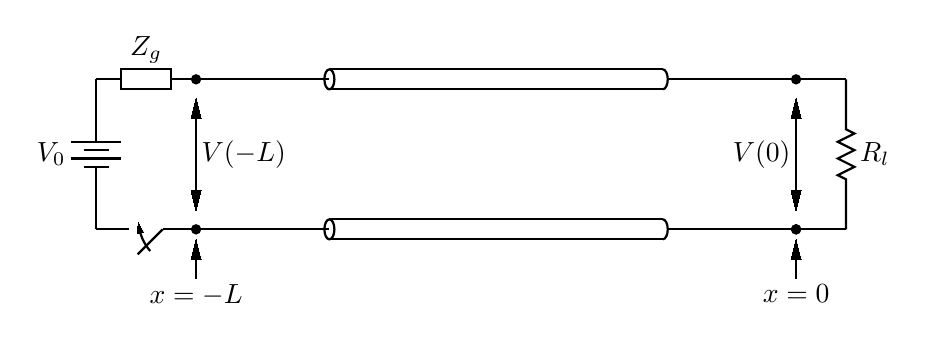
\begin{tikzpicture}[scale=2.54]
% dpic version 2010.11.28 option -g for TikZ and PGF 1.01
\ifx\dpiclw\undefined\newdimen\dpiclw\fi
\global\def\dpicdraw{\draw[line width=\dpiclw]}
\global\def\dpicstop{;}
\dpiclw=0.8bp
\dpiclw=0.8bp
\dpicdraw (0,0)
 --(0,0.3125)\dpicstop
\dpicdraw (-0.0625,0.3125)
 --(0.0625,0.3125)\dpicstop
\dpicdraw (-0.125,0.354167)
 --(0.125,0.354167)\dpicstop
\dpicdraw (-0.0625,0.395833)
 --(0.0625,0.395833)\dpicstop
\dpicdraw (-0.125,0.4375)
 --(0.125,0.4375)\dpicstop
\dpicdraw (0,0.4375)
 --(0,0.75)\dpicstop
\draw (-0.125,0.375) node[left=-1.5bp]{$V_0$};
\dpicdraw (0,0.75)
 --(0.125,0.75)\dpicstop
\dpicdraw (0.375,0.75)
 --(0.375,0.8)
 --(0.125,0.8)
 --(0.125,0.7)
 --(0.375,0.7)
 --(0.375,0.75)\dpicstop
\dpicdraw (0.375,0.75)
 --(0.5,0.75)\dpicstop
\draw (0.25,0.8) node[above=-1.5bp]{$ Z_g$};
\dpicdraw[fill=black](0.5,0.75) circle (0.007874in)\dpicstop
\dpicdraw[fill=black](0.5,0) circle (0.007874in)\dpicstop
\filldraw[line width=0bp](0.525,0.55625)
 --(0.5,0.65625)
 --(0.475,0.55625) --cycle
\dpicstop
\dpicdraw (0.5,0.633344)
 --(0.5,0.19375)\dpicstop
\filldraw[line width=0bp](0.475,0.19375)
 --(0.5,0.09375)
 --(0.525,0.19375) --cycle
\dpicstop
\draw (0.5,0.375) node[right=-1.5bp]{$V(-L)$};
\dpicdraw (2.858333,0.75)
 --(3.5,0.75)\dpicstop
\dpicdraw (0.5,0.75)
 --(1.166667,0.75)\dpicstop
\dpicdraw (1.166667,0.7)
 --(2.833333,0.7)\dpicstop
\dpicdraw (2.833333,0.7)
 ..controls (2.847141,0.7) and (2.858333,0.722385)
 ..(2.858333,0.75)
 ..controls (2.858333,0.777615) and (2.847141,0.8)
 ..(2.833333,0.8)\dpicstop
\dpicdraw (2.833333,0.8)
 --(1.166667,0.8)\dpicstop
\dpicdraw (1.166667,0.8)
 ..controls (1.152859,0.8) and (1.141667,0.777615)
 ..(1.141667,0.75)
 ..controls (1.141667,0.722385) and (1.152859,0.7)
 ..(1.166667,0.7)
 ..controls (1.180474,0.7) and (1.191667,0.722385)
 ..(1.191667,0.75)
 ..controls (1.191667,0.777615) and (1.180474,0.8)
 ..(1.166667,0.8)\dpicstop
\dpicdraw[fill=black](3.5,0.75) circle (0.007874in)\dpicstop
\dpicdraw[fill=black](3.5,0) circle (0.007874in)\dpicstop
\filldraw[line width=0bp](3.525,0.55625)
 --(3.5,0.65625)
 --(3.475,0.55625) --cycle
\dpicstop
\dpicdraw (3.5,0.633344)
 --(3.5,0.19375)\dpicstop
\filldraw[line width=0bp](3.475,0.19375)
 --(3.5,0.09375)
 --(3.525,0.19375) --cycle
\dpicstop
\draw (3.5,0.375) node[left=-1.5bp]{$V(0)$};
\dpicdraw (3.5,0.75)
 --(3.75,0.75)\dpicstop
\dpicdraw (3.75,0.75)
 --(3.75,0.5)
 --(3.791667,0.479167)
 --(3.708333,0.4375)
 --(3.791667,0.395833)
 --(3.708333,0.354167)
 --(3.791667,0.3125)
 --(3.708333,0.270833)
 --(3.75,0.25)
 --(3.75,0)\dpicstop
\draw (3.791667,0.375) node[right=-1.5bp]{$ R_l$};
\dpicdraw (3.75,0)
 --(3.5,0)\dpicstop
\dpicdraw[fill=black](3.5,0) circle (0.007874in)\dpicstop
\dpicdraw (2.858333,0)
 --(3.5,0)\dpicstop
\dpicdraw (0.5,0)
 --(1.166667,0)\dpicstop
\dpicdraw (1.166667,-0.05)
 --(2.833333,-0.05)\dpicstop
\dpicdraw (2.833333,-0.05)
 ..controls (2.847141,-0.05) and (2.858333,-0.027615)
 ..(2.858333,0)
 ..controls (2.858333,0.027615) and (2.847141,0.05)
 ..(2.833333,0.05)\dpicstop
\dpicdraw (2.833333,0.05)
 --(1.166667,0.05)\dpicstop
\dpicdraw (1.166667,0.05)
 ..controls (1.152859,0.05) and (1.141667,0.027615)
 ..(1.141667,0)
 ..controls (1.141667,-0.027615) and (1.152859,-0.05)
 ..(1.166667,-0.05)
 ..controls (1.180474,-0.05) and (1.191667,-0.027615)
 ..(1.191667,0)
 ..controls (1.191667,0.027615) and (1.180474,0.05)
 ..(1.166667,0.05)\dpicstop
\dpicdraw (0.5,0)
 --(0.333333,0)\dpicstop
\dpicdraw (0.333333,0)
 --(0.208333,-0.125)\dpicstop
\filldraw[line width=0bp](0.221268,-0.018447)
 --(0.237529,-0.01371)
 ..controls (0.227538,0.000674) and (0.219175,0.016123)
 ..(0.212593,0.032352)
 ..controls (0.207874,0.014206) and (0.205327,-0.004436)
 ..(0.205006,-0.023183)
 --(0.221268,-0.018447)\dpicstop
\dpicdraw (0.217461,-0.002327)
 ..controls (0.225975,-0.041593) and (0.244342,-0.078046)
 ..(0.270833,-0.108253)\dpicstop
\dpicdraw (0.166667,0)
 --(0,0)\dpicstop
\filldraw[line width=0bp](0.525,-0.15)
 --(0.5,-0.05)
 --(0.475,-0.15) --cycle
\dpicstop
\dpicdraw (0.5,-0.072906)
 --(0.5,-0.25)\dpicstop
\draw (0.5,-0.25) node[below=-1.5bp]{$x=-L$};
\filldraw[line width=0bp](3.525,-0.15)
 --(3.5,-0.05)
 --(3.475,-0.15) --cycle
\dpicstop
\dpicdraw (3.5,-0.072906)
 --(3.5,-0.25)\dpicstop
\draw (3.5,-0.25) node[below=-1.5bp]{$x=0$};
\end{tikzpicture}
\caption{Fuente de corriente directa que alimenta una l�nea de transmisi�n sin p�rdidas, que acopla una carga netamente resistiva $R_l$.}
\label{fig:FueCCMasIntMasLTxMasRes}
\end{figure}
\end{document}
